%%%%%%%%%%%%%%%%%%%%%%%%%%%%%%%%%%%%%%
%%%%%%%%%%%%%%%%%%%%%%%%%%%%%%%%%%%%%%
% Do not edit the TeX file your work
% will be overwritten.  Edit the RnW
% file instead.
%%%%%%%%%%%%%%%%%%%%%%%%%%%%%%%%%%%%%%
%%%%%%%%%%%%%%%%%%%%%%%%%%%%%%%%%%%%%%



The left plot of \figref{example_genes}
shows the measurements of a single gene over time.
We model each gene as belonging to a latent component,
where each component defines a smooth expression curve over time.
Then, observations are drawn by adding i.i.d.\ noise to the smoothed
curve along with a gene-specific offset.
Following \citet{Luan:2003:clustering}, we construct the smoothers
using cubic B-splines.

Let $\x_\n\in\mathbb{R}^\ntimepoints$ be measurements of gene $\n$ at
$\ntimepoints$ time points. Let $\regmatrix$ be the $\ntimepoints \times \d$
B-spline regressor matrix, so that the $ij$-th entry of $\regmatrix$ is the
$j$-th B-spline basis vector evaluated at the $i$-th time point. The right plot
of \figref{example_genes} shows the B-spline basis. 


\begin{knitrout}
\definecolor{shadecolor}{rgb}{0.969, 0.969, 0.969}\color{fgcolor}\begin{figure}[!h]

{\centering 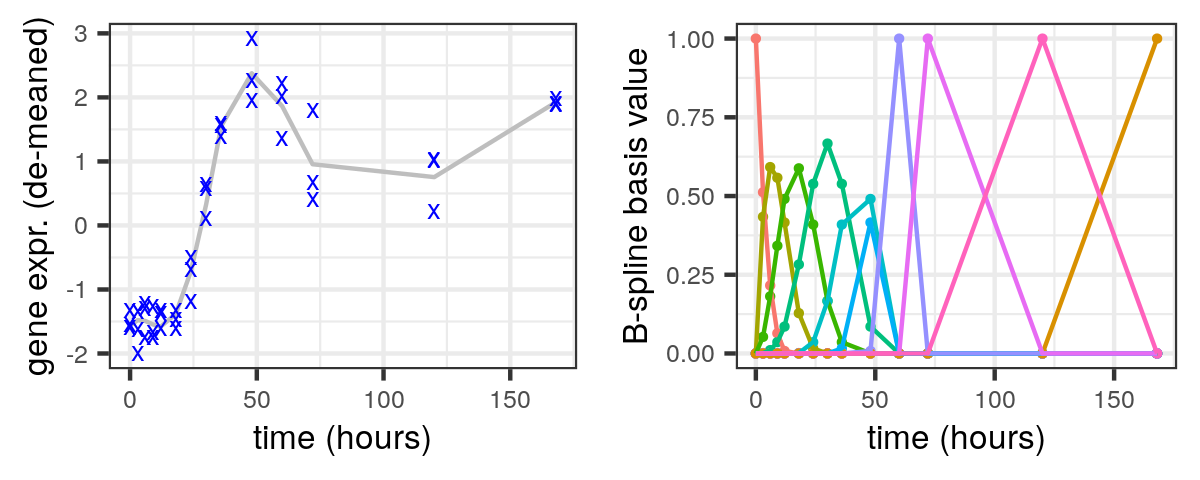
\includegraphics[width=0.980\linewidth,height=0.392\linewidth]{figure/example_genes-1} 

}

\caption[(Left) An example gene and its expression measured at 14 unique time points
    with three biological replicates at each time point.
     (Right) The cubic B-spline basis with 7 degrees of freedom,
    along with three indicator functions for the last three time points,
    $\timeindx = 72, 120, 168$]{(Left) An example gene and its expression measured at 14 unique time points
    with three biological replicates at each time point.
     (Right) The cubic B-spline basis with 7 degrees of freedom,
    along with three indicator functions for the last three time points,
    $\timeindx = 72, 120, 168$.}\label{fig:example_genes}
\end{figure}


\end{knitrout}
%
